\section*{Appendix}

\begin{subappendices}
\section{Parameter Estimation}
\label{c2:appendix:A}
We estimate parameters of the joint model using Markov chain Monte Carlo (MCMC) methods under the Bayesian framework. Let $\boldsymbol{\theta}$ denote the vector of the parameters of the joint model. The joint model postulates that given the random effects, time to GR and longitudinal responses taken over time are all mutually independent. Under this assumption the posterior distribution of the parameters is given by:
\begin{align*}
p(\boldsymbol{\theta}, \boldsymbol{b} \mid \mathcal{D}_n) & \propto \prod_{i=1}^n p(l_i, r_i, \boldsymbol{y}_i \mid \boldsymbol{b}_i, \boldsymbol{\theta}) p(\boldsymbol{b}_i \mid \boldsymbol{\theta}) p(\boldsymbol{\theta})\\
& \propto \prod_{i=1}^n p(l_i, r_i \mid \boldsymbol{b}_i, \boldsymbol{\theta}) p(\boldsymbol{y}_i \mid \boldsymbol{b}_i, \boldsymbol{\theta}) p(\boldsymbol{b}_i \mid \boldsymbol{\theta}) p(\boldsymbol{\theta}),\\
p(\boldsymbol{b}_i \mid \boldsymbol{\theta}) &= \frac{1}{\sqrt{(2 \pi)^q \text{det}(\boldsymbol{D})}} \exp(\boldsymbol{b}_i^T \boldsymbol{D}^{-1} \boldsymbol{b}_i),
\end{align*}
where the likelihood contribution of longitudinal outcome conditional on random effects is:
\begin{align*}
p(\boldsymbol{y}_i \mid \boldsymbol{b}_i, \boldsymbol{\theta}) &= \frac{1}{\big(\sqrt{2 \pi \sigma^2}\big)^{n_i}} \exp\bigg(-\frac{{\lVert{\boldsymbol{y}_i - \boldsymbol{X}_i\boldsymbol{\beta} - \boldsymbol{Z}_i\boldsymbol{b}_i}\rVert}^2}{\sigma^2}\bigg),\\
\boldsymbol{X}_i &= \{\boldsymbol{x}_i(t_{i1})^T, \ldots, \boldsymbol{x}_i(t_{in_i})^T\}^T,\\
\boldsymbol{Z}_i &= \{\boldsymbol{z}_i(t_{i1})^T, \ldots, \boldsymbol{z}_i(t_{in_i})^T\}^T.
\end{align*}
The likelihood contribution of the time to GR outcome is given by:
\begin{equation}
\label{c2:eq:likelihood_survival_part}
\begin{split}
p(l_i,r_i\mid \boldsymbol{b}_i,\boldsymbol{\theta}) &= \exp\Big\{-\int_0^{l_i} h_i(s \mid \mathcal{M}_i(s), \boldsymbol{w}_i)\mathrm{d}{s}\Big\} \\ & \quad - \exp\Big\{-\int_0^{r_i}h_i(s \mid \mathcal{M}_i(s), \boldsymbol{w}_i)\mathrm{d}{s}\Big\}.
\end{split}
\end{equation}
The integral in (\ref{c2:eq:likelihood_survival_part}) does not have a closed-form solution, and therefore we use a 15-point Gauss-Kronrod quadrature rule to approximate it.

We use independent normal priors with zero mean and variance 100 for the fixed effects $\boldsymbol{\beta}$, and inverse Gamma prior with shape and rate both equal to 0.01 for the parameter $\sigma^2$. For the variance-covariance matrix $\boldsymbol{D}$ of the random effects, we take inverse Wishart prior with an identity scale matrix and degrees of freedom equal to $q$ (number of random effects). For the relative risk model's parameters $\boldsymbol{\gamma}$ and the association parameters $\boldsymbol{\alpha}$, we use independent normal priors with zero mean and variance 100.

\subsection{Parameter Estimates}
The longitudinal evolution of $\log_2 (\mbox{PSA} + 1)$ is modeled with non-linear terms. Hence, the interpretation of the coefficients in this model is not straightforward. Instead of the parameter estimates, in Figure~\ref{c2:fig:app1}, we present the fitted marginal evolution of $\log_2 (\mbox{PSA} + 1)$ over a period of 10 years for a hypothetical patient who is included in AS at the age of 70 years. 

%In addition we present plots of observed versus fitted PSA profiles for nine randomly selected PRIAS patients in Figure~\ref{c2:fig:app2}. Lastly, the quantile-quantile plot of subject-specific residuals in Figure~\ref{c2:fig:app3} shows that the assumption of t-distributed (df=3) errors is reasonably met by the fitted model.

\begin{figure}
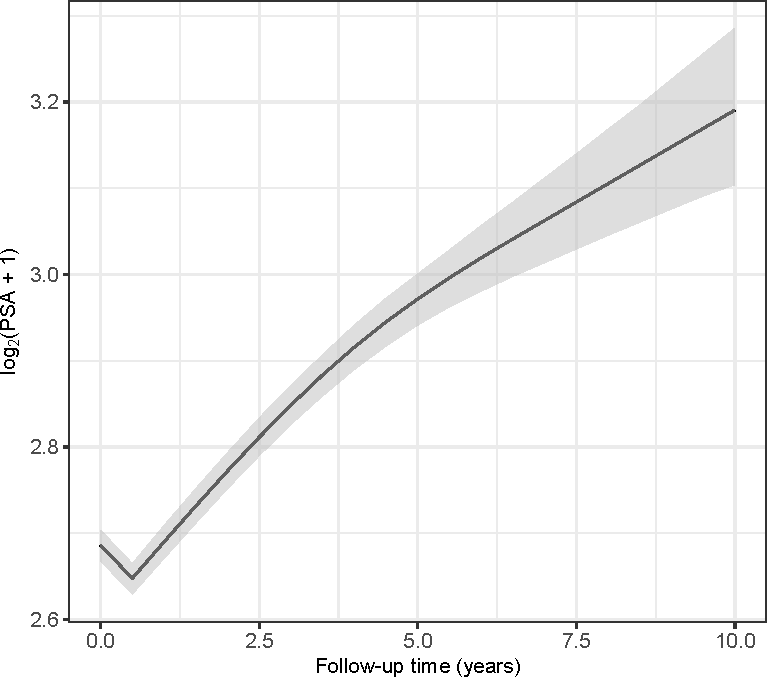
\includegraphics{contents/c2/images/c2_fig_app1.pdf}
\caption{\textbf{Fitted marginal evolution} of $\log_2(\mbox{PSA} + 1)$ measurements over a period of 10 years with 95\% credible interval, for a hypothetical patient who is included in AS at the age of 70 years.}
\label{c2:fig:app1}
\end{figure}

%\begin{figure}
%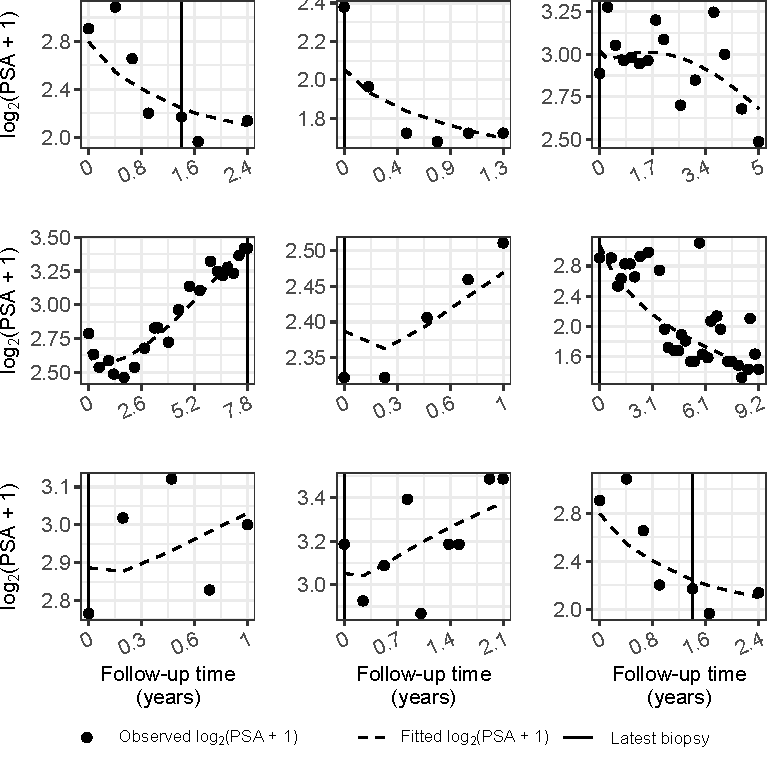
\includegraphics{contents/c2/images/c2_fig_app2.pdf}
%\caption{\textbf{Fitted versus observed} ${\log_2(\mbox{PSA} + 1)}$ profiles for nine randomly selected PRIAS patients. The fitted profiles utilize information from the observed PSA measurements, and time of the latest biopsy.}
%\label{c2:fig:app2}
%\end{figure}

%\begin{figure}
%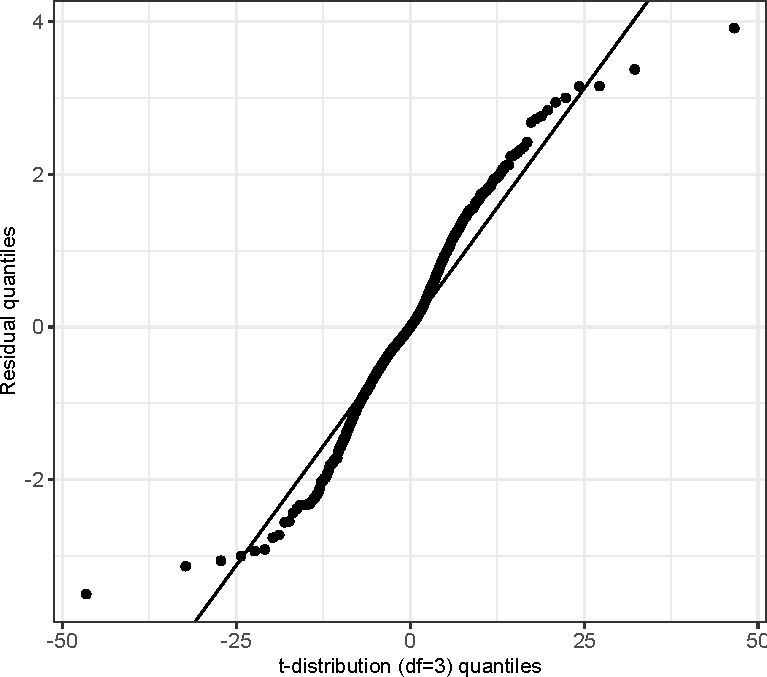
\includegraphics{contents/c2/images/c2_fig_app3.pdf}
%\caption{\textbf{Quantile-quantile plot} of subject-specific residuals of PSA obtained from the joint model fitted to the PRIAS dataset.}
%\label{c2:fig:app3}
%\end{figure}

For the relative risk sub-model, the parameter estimates in Table~\ref{c2:table:app1} show that ${\log_2 (\mbox{PSA} + 1)}$ velocity and the age at the time of inclusion in AS are strongly associated with the hazard of GR. For any patient, an increase in $\log_2 (\mbox{PSA} + 1)$ velocity from -0.061 to 0.136 (first and third quartiles of the fitted velocities, respectively) corresponds to a 2.046 fold increase in the hazard of GR. An increase in age at the time of inclusion in AS from 65 years to 75 years (first and third quartiles of age in PRIAS dataset) corresponds to a 1.428 fold increase in the hazard of GR.

\begin{table}
\small
\centering
\caption{\textbf{Parameters of the relative-risk sub-model}: Estimated mean and 95\% credible interval. Age is median centered.}
\label{c2:table:app1}
\begin{tabular}{lrrrrr}
\toprule
Variable                      & Mean   & Std. Dev & 2.5\%  & 97.5\%                 & P              \\ 
\midrule
$(\mbox{Age} - 70)$                  & 0.036 & 0.006 & 0.024 & 0.047 & \textless0.000 \\
$(\mbox{Age} - 70)^2$   & -0.001 & 0.001 & -0.003 & 7.861 $\times 10^{-5}$ & 0.084          \\
$\log_2 (\mbox{PSA} + 1)$                  & -0.084 & 0.080 & -0.241 & 0.072 & 0.296         \\
Slope($\log_2 (\mbox{PSA} + 1)$)           & 3.580 & 0.403 & 2.815 & 4.373 & \textless0.000 \\
\bottomrule
\end{tabular}
\end{table}

\section{Ascertainment Bias: PSA Doubling Time-Dependent Biopsies and Competing Events}
\label{c2:appendix:B}
\textbf{PSA dependent interval-censored time of upgrading:} The true time of upgrading $T^*_i$ is not known for any of the patients in PRIAS. To detect upgrading, PRIAS uses a fixed schedule of biopsies wherein biopsies are conducted at year one, year four, year seven and year ten of follow-up, and every five years after that. However, PRIAS switches to a more frequent annual biopsy schedule for faster-progressing patients. These are patients with PSA doubling time (PSA-DT) between 0 and 10 years, which is measured as the inverse of the slope of the regression line through the base two logarithm of PSA values. Thus, the interval $l_i < T_i^* \leq r_i$ in which upgrading is detected depends on the observed PSA values. 

\textbf{Competing events:} The primary event of interest in this paper is upgrading observed via a positive biopsy. There are three types of competing events, namely death, removal of patients from AS on the basis of their observed DRE and PSA measurements, watchful-waiting, and loss to follow-up of patients because of patient anxiety or unknown reasons.

The number of patients obtaining the event death is small compared to the number of patients who obtain the primary event upgrading. Hence in this paper, considering death as non-informative censoring may be viable. We also consider the loss to follow-up as non-informative censoring, which may not always be true. This is especially the case when the reason for loss to follow-up is unknown. However, when the reason for loss to follow-up is patient anxiety, it is often on the basis of their observed results. Given the large number of loss to follow-up patients, considering these patients as censored is a limitation of our work. However, the problem of the unknown reason for dropout is not specific to only our model. For the remaining patients who are removed from AS on the basis of their observed longitudinal data (e.g., treatment, watchful-waiting), in the next paragraph, we show that the removal of these patients is non-informative about the parameters of the model for the true time of upgrading.

Given the aforementioned issues of PSA dependent interval censoring and removal of patients on the basis of their observed longitudinal data is natural to question in this scenario if the parameters of the joint model are affected by these two. However, because the parameters of the joint model are estimated using a full likelihood approach~\citep{tsiatis2004joint}, the joint model allows the schedule of biopsies, as well as censoring to depend upon the observed PSA measurements (e.g., via PSA-DT), under the condition that the model is correctly specified. To show this, consider the following full general specification of the joint model that we use. Let $\boldsymbol{y}_i$ denote the observed PSA measurements for the $i$-th patient, and $l_i, r_i$ denote the two time points of the interval in which upgrading occurs for the $i$-th patient. In addition, let $T_i^S$ and $\mathcal{V}_i$ denote the schedule of biopsies, and the schedule PSA measurements, respectively. Let $G^*_i$ denote the time of removal from AS without observing upgrading. Under the assumption that $T_i^S, G^*_i, \mathcal{V}_i$ may depend upon only the observed data $\boldsymbol{y}_i$, the joint likelihood of the various processes is given by:
\begin{equation*}
p(\boldsymbol{y}_i, l_i, r_i, T_i^S, G^*_i, \mathcal{V}_i \mid \boldsymbol{\theta}, \boldsymbol{\psi}) = p(\boldsymbol{y}_i, l_i, r_i \mid \boldsymbol{\theta}) \times p(T_i^S, G^*_i, \mathcal{V}_i \mid \boldsymbol{y}_i, \boldsymbol{\psi}).
\end{equation*}
where, $\boldsymbol{\psi}$ is the vector of parameters for the processes $T_i^S, G^*_i, \mathcal{V}_i$. From this decomposition, we can see that even if the processes $T_i^S, G^*_i, \mathcal{V}_i$ may be determined from $\boldsymbol{y}_i$, if we are interested in the parameters $\boldsymbol{\theta}$ of the joint distribution of longitudinal and event outcomes, we can maximize the likelihood based on the first term and ignore the second term. In other words, the second term will not carry information for $\boldsymbol{\theta}$. Lastly, since we use a full likelihood approach with an interval censoring specification, the estimates that we obtain are consistent and asymptotically unbiased \citep{gentleman1994maximum}, despite the interval censoring observed. 

We also demonstrate the validity of our argument via a simulated dataset of 750 patients. The true event times $T^*_i$ for these patients were generated using parameters from a joint model fitted to the PRIAS dataset (with the only change that $\log_2 \mbox{PSA}$ levels are used as the outcome). However, this joint model did not include the association between the velocity of log PSA values and the hazard of GR. That is, the hazard of GR $h_i(t)$ at any time $t$ was dependent only on the underlying $\log_2 \mbox{PSA}$ value $m_i(t)$ at that time. Furthermore, for these patients, we used the schedule of PRIAS to generate the interval $l_i \leq T^*_i \leq r_i$ in which GR is detected. Thus the observed data for $i$-th patient is $\{\boldsymbol{y}_i, l_i, r_i\}$. Our aim is to show that if there is no association between $h_i(t)$ and velocity of log PSA value $m'_i(t)$, then even though the biopsy schedule depends on PSA-DT (which is a crude measure of PSA velocity), a joint model fitted with both value and velocity associations will have an insignificant velocity association. In the fitted joint model, we found the value association (95\% credible interval in brackets) to be 0.182~[0.090,~0.274], and the velocity association to be -0.001~[-0.295,~0.254]. That is, even though the schedule of biopsies depended upon observed PSA values, it did not lead to a spurious velocity association. 

\section{Source Code}
The source code for fitting the joint model is available at \url{https://raw.githubusercontent.com/anirudhtomer/prias/master/src/chapter2_biometricspaper/Gleason%20as%20event/log2psaplus1_and_pluspt1.R}. 

The code generating the simulation population is available at \url{https://github.com/anirudhtomer/prias/blob/master/src/chapter2_biometricspaper/simulation_study/SimulateJM.R}. 

The code for scheduling biopsies using fixed schedules and utility functions is available at \url{https://github.com/anirudhtomer/prias/blob/master/src/chapter2_biometricspaper/simulation_study/nbAndOffset.R}.

\end{subappendices}